\documentclass[graphics]{beamer}
\usepackage{xcolor}
\usepackage{graphicx}
\usepackage{verbatim}
\usepackage{wrapfig}
\useoutertheme{shadow}
%\usecolortheme{orchid}
\usecolortheme{seahorse}


% math commands
\newcommand{\be}{\begin{eqnarray}}
\newcommand{\ee}{\end{eqnarray}}
\newcommand{\beq}{\begin{equation}}
\newcommand{\eeq}{\end{equation}}
\def\simless{\mathbin{\lower 3pt\hbox
      {$\rlap{\raise 5pt\hbox{$\char'074$}}\mathchar"7218$}}}
\def\simgreat{\mathbin{\lower 3pt\hbox
      {$\rlap{\raise 5pt\hbox{$\char'076$}}\mathchar"7218$}}} %> or of order

% variables

\def\toonscale{0.45}
\def\mboxy#1{\mbox{\small #1}}

\defbeamertemplate*{title page}{customized}[1][]
{
  \usebeamerfont{title}\inserttitle\par
  \usebeamerfont{subtitle}\usebeamercolor[fg]{subtitle}\insertsubtitle\par
  \bigskip
  \usebeamerfont{author}\insertauthor\par
  \usebeamerfont{institute}\insertinstitute\par
  \usebeamerfont{date}\insertdate\par
  \usebeamercolor[fg]{titlegraphic}\inserttitlegraphic
}
\begin{comment}
\AtBeginSection[]{
  \frame{
    \frametitle{Outline}
    \tableofcontents[currentsection]
  }
}
\end{comment}


\title{New Scintillometry Windows}
%\subtitle{}
\author[U. Pen]{{
\textcolor{green}{\small Dana Simard, Robert Main, Daniel Baker}, 
\textcolor{cyan}{\small I-Sheng Yang, Franz Kirsten} 
\textcolor{darkgray}{\small U. Pen, M. van Kerkwijk, K. Vanderlinde, J-P Macquart and many more}
}
\\[8mm] 
}
\date{September 20, 2016}


\begin{document}

\frame{
\vspace{-0.5in}
\begin{center}  
%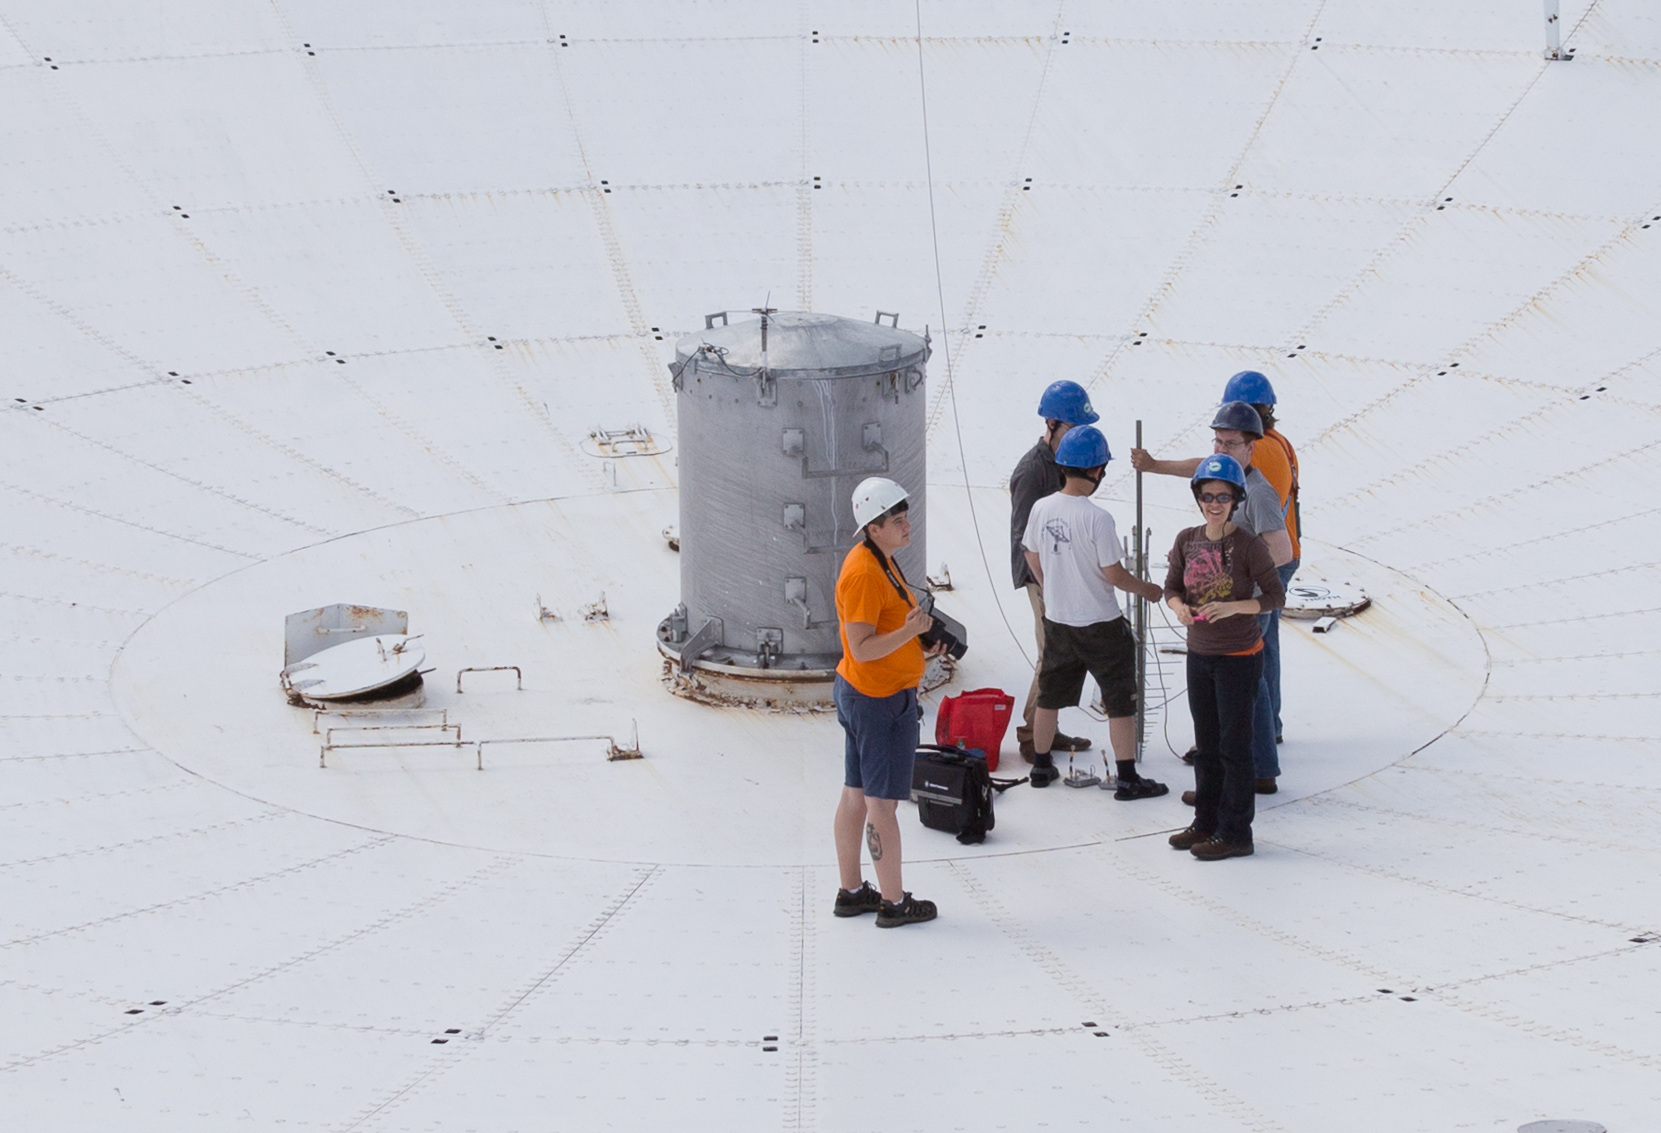
\includegraphics[width=4.4in]{Figures/IMG-0438-by-Andre-cropped.jpg}
\end{center}
\begin{picture}(320,250)
\put(-50,60){
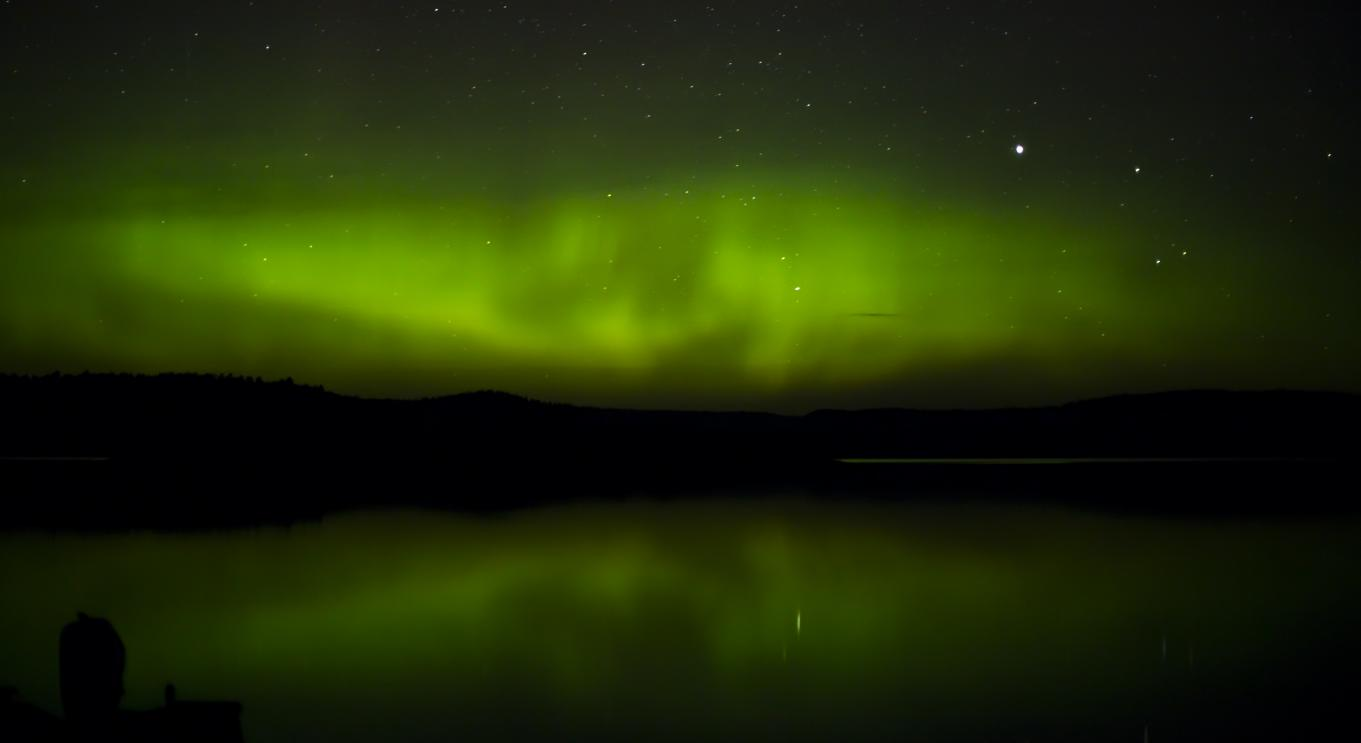
\includegraphics[width=5.5in]{Figures/traverse-aurora.jpg}}
\end{picture}
\vspace{-4in}
\\
image credit: Andre Recnik
\\
\vspace{1in}
\titlepage
}

%\section*{Introduction}
\section{Introduction}

\begin{comment}
  \subsection{Outline}

  \frame{
    \frametitle{Outline}
    \tableofcontents
  }
\end{comment}


\section{Overview}

\frame{
    \frametitle{Facts}
    \begin{itemize}
      \item Test alternative gravity
      \item increase PTA sensivity, angular resolution
      \item resolve FRB environment
    \end{itemize}

}

\frame{
    \frametitle{FRB environment}
    \begin{itemize}
      \item FRB1105023 shows scintillation coherent across scattering tail
      \item proves that scattering is not from ISM
    \end{itemize}

}
\frame{
    \frametitle{PTA sensivity}
    \begin{itemize}
      \item measure pulsar distance to better than GW wavelength (see other talks)
      \item combine pulsar term and earth term coherently
      \item equivalent to doubling sensitivity
    \end{itemize}
}

\frame{
    \frametitle{PTA angular resolution}
    \begin{itemize}
      \item commonly viewed as 'stochastic background'
      \item with distance information, resolution is $\theta\lambda/D$, with
        GW $\lambda \sim $ly and $D$ distance to pulsar several
        thousand ly
      \item resolution $\sim$ arc minutes (Boyle+UP 2012)
        \item no source confusion, opens window for optical
          identification
    \end{itemize}
}



\end{document}
